% ****** Start of file apssamp.tex ******
%
%   This file is part of the APS files in the REVTeX 4.2 distribution.
%   Version 4.2a of REVTeX, December 2014
%
%   Copyright (c) 2014 The American Physical Society.
%
%   See the REVTeX 4 README file for restrictions and more information.
%
% TeX'ing this file requires that you have AMS-LaTeX 2.0 installed
% as well as the rest of the prerequisites for REVTeX 4.2
%
% See the REVTeX 4 README file
% It also requires running BibTeX. The commands are as follows:
%
%  1)  latex apssamp.tex
%  2)  bibtex apssamp
%  3)  latex apssamp.tex
%  4)  latex apssamp.tex
%
\documentclass[%
 reprint,
%superscriptaddress,
%groupedaddress,
%unsortedaddress,
%runinaddress,
%frontmatterverbose, 
%preprint,
%preprintnumbers,
%nofootinbib,
%nobibnotes,
%bibnotes,
 amsmath,amssymb,
 aps, 
%pra,
%prb,
%rmp,
%prstab,
%prstper,
%floatfix,
]{revtex4-2}

\usepackage{hyperref}
\hypersetup{
    colorlinks=true,
    linkcolor=blue,
    filecolor=blue,      
    urlcolor=blue,
    citecolor=blue,
}
\usepackage[ruled,vlined]{algorithm2e}

\usepackage{physics}
\usepackage{fixme}
%\usepackage{algorithm}
\usepackage{algorithmic}
\usepackage{graphicx}% Include figure files
\usepackage{dcolumn}% Align table columns on decimal point
\usepackage{bm}% bold math
%\usepackage{hyperref}% add hypertext capabilities
%\usepackage[mathlines]{lineno}% Enable numbering of text and display math
%\linenumbers\relax % Commence numbering lines

%\usepackage[showframe,%Uncomment any one of the following lines to test 
%%scale=0.7, marginratio={1:1, 2:3}, ignoreall,% default settings
%%text={7in,10in},centering,
%%margin=1.5in,
%%total={6.5in,8.75in}, top=1.2in, left=0.9in, includefoot,
%%height=10in,a5paper,hmargin={3cm,0.8in},
%]{geometry}

\begin{document}

\preprint{APS/123-QED}

\title{Correlation between different emission channels from an atom inside a leaky driven cavity}% Force line breaks with \\

\author{Guillermo Preisser}
 \email{Corresponding author e-mail: guillermo.preisser@uabc.edu.mx}
 %Lines break automatically or can be forced with \\
\author{Pablo Barberis}%
\affiliation{Instituto de Investigaciones en Matemáticas Aplicadas y en Sistemas, Universidad Nacional Autónoma de México, Ciudad Universitaria, 04510, CDMX, México.}



\date{\today}% It is always \today, today,
             %  but any date may be explicitly specified

\begin{abstract}
A two level atom in free space does not show any correlation between
  photons emitted in different directions. We consider a two level
  atom inside a driven leaky cavity. We consider two atomic emission
  channels: emission to cavity modes and emission to no-cavity modes.
  Using the quantum trajectory formalism we study the correlation
  between photons emitted into cavity modes and that leak the cavity
  through its mirror, with photons that are emitted into the rest of
  the modes. We find that the cavity generates a correlation between
  the two emission channels.
\end{abstract}

%\keywords{Suggested keywords}%Use showkeys class option if keyword
                              %display desired
\maketitle

%\tableofcontents

\section{INTRODUCTION}

Spontaneous emission is a phenomenon that has been studied since the
early XX century \cite{10.2307/94746, 1917PhyZ...18..121E}. One of the
main characteristics of spontaneous emission is that
\fxnote{spontaneus emission no es exponencial, es aproximadamente
  exponencial, si quitas la aproximacion markoviana te queda una cola
  polinomial, quite la oracion} the exact time of emission, as well as
the direction in which the photon is emitted, is random, which
difficults its measurement. On the other hand, photons emitted from a
cavity are easy to measure, partly due the fact that we know that they
leave the cavity through one of the lateral mirrors \cite{326305,
  doi:10.1063/1.113345}. The randomness of the direction in which the
photons are emitted by atoms in free space difficults photon counting
experiments. To sort out this difficulty one could think of a physical
arrangement, in which the two-level atom is coupled to the stimulated
mode of a cavity, as it is shown in Fig. \ref{asa} (b). In this
physical arrangement, \fxnote*{tienes una cita donde lo nombren
  asi?}{which is known as the driven Jaynes-Cummings model}, one could
try to estimate the number of spontaneous emissions of the atom
--which are emitted in modes that are not cavity modes and therefore
escape the cavity-- by measuring the photons that leak through one of
the cavity mirrors. In the case that a
correlation exists between the two quantities, we can count the number
of photons that leak the cavity through its mirror, which is easy to
measure, to find information about the number of photons emitted into
the other modes (spontaneus emission), which are difficult to measure.

In the case of a two-level atom in free space, the absence of
correlation between different channels is the result of the markovian
approximation, which assumes that the environment has no memory of
previous interactions with the system \cite{daley2014quantum}. Two
atomic emissions would be correlated if one of the emissions stay
registered in the environment and, somehow, influence the second
emission of a two-level atom at a later time; the Markovian
approximation does not allow memory effects and there is no
correlation between the number of emissions of each source: knowing
the number of photons emitted in some region of the space during some
time does not give me any information on the number of photons emitted
in other region of the space. Nevertheless, for the case of an atom
inside a cavity, before a photon leaks the cavity, it will interact
with the atom for some time. This interaction with the atom before the
emission generates a correlation between photons that leak the cavity
through its mirror and photons that leak the cavity through its side.

We use quantum trajectory theory to theoretically calculate the
correlation between different emission channels. A quantum trajectory
is the description of a continuously monitored quantum system
conditioned on a particular past history of coherent evolution and
collapse \cite{Carmichael1993Open}. These trajectories are simulated
through a stochastic process, which define the times when the
collapses occur. Each trajectory gives us the number of photon emitted
in each channel. Simulating a large number of trajectories and
registering the number of photon emissions into the two channels, we
obtain its correlation. The correlation varies with the cavity
linewidth and the atom-cavity coupling. For a very bad cavity we
recover the free space result: there is no correlation between the two
channels.


This article is organized as follows: A general overview of the driven
Jaynes-Cummings model is presented in section \ref{sc:drivenjc}. In
section \ref{sc:distributions} we obtain probability distributions
that relate the number of spontaneous and cavity emissions. In section
\ref{sc:correlation} we calculate the correlation between the two variables.
Concluding remarks are given in section \ref{sc:conclusions}
\begin{center}
\begin{figure*}\label{asa}
\begin{center}
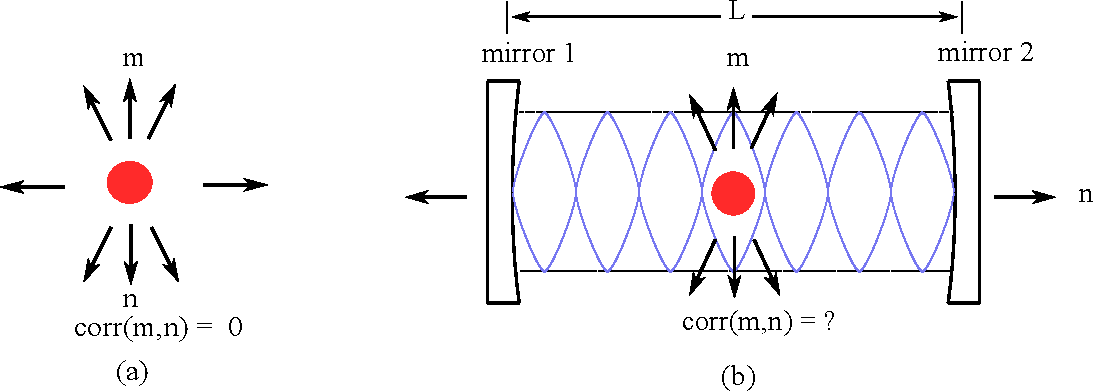
\includegraphics[scale = 0.65]{newimagepaper.pdf}
%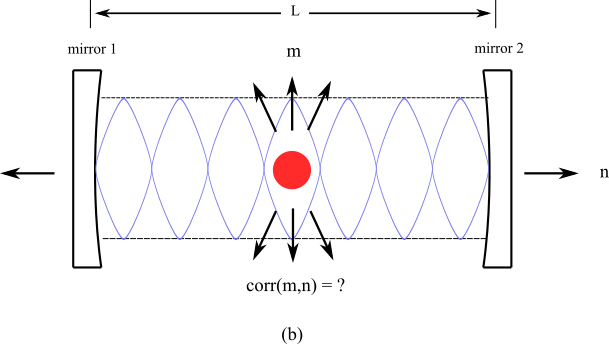
\includegraphics[scale = 0.45]{image_paper222.png}
\caption{\small{Physical arrangements of atom and atom in a cavity. In
    both of these arrangements we consider a source which stimulates
    the atom provoking it to spontaneously emit, once it decays. We
    consider a detector in two directions, and we keep a register of
    the number of photons measured in each direction. (a) In the case
    for the atom we don't expect a correlation between m (the number
    of photons measured in the upper side of the atom) and n (the
    number of photons measured in the right side of the atom); (b) for
    the atom in the cavity (a cavity with some loss rate) we study the
    possibility that the cavity generates a correlation between the
    emissions of the atom and the emissions of the cavity, which
    correspond to the emissions that leak through mirror
    2.}} 
\end{center}
\end{figure*}
\end{center}


\section{Driven Jaynes-Cummings model}\label{sc:drivenjc}
e consider a system consisting of a two-level atom, coupled to a mode
of a leaky cavity. The mode is driven by a coherent field resonant
with the atomic transition and the cavity mode.
% In order to account for
% dissipation one may use a non-hermitian Hamiltonian to describe the
% system \cite{bla}. Using this description for the system will turn
% useful at the moment of using quantum trajectory theory. Such
% Hamiltonian can be separated into hermitian and non-hermitian terms.
%\begin{equation}
%H = H_s - \frac{i\hbar}{2}\sum_m C^\dagger_n C_n .
%\end{equation}
The Hamiltonian of this system, in the rotating wave approximation is
given by
\begin{equation}
H_s = H_{at} + H_{cav} + H_{atcav} + H_{lascav}, \label{mainham}  
\end{equation}
where the atom and cavity terms are, respectively
\begin{subequations}
\begin{equation}
H_{at} = \tfrac{1}{2}\hbar \omega \sigma_z,    
\end{equation}
\begin{equation}
H_{cav} = \hbar \omega  a^\dagger a,  
\end{equation}
while the coupling between atom and cavity, and cavity and coherent
field are
\begin{equation}
H_{atcav} = i\hbar g(a\sigma_+ - a^\dagger \sigma_-),    
\end{equation}
\begin{equation}
H_{lascav} = i\hbar \mathcal{E}(ae^{i\omega t} - a^\dagger e^{-i\omega t}),    
\end{equation}
\end{subequations}
where the annihilation operator $a$ of a single photon in the cavity,
and the creation operator $a^\dagger$ obey $[a, a^\dagger] = 1$. The
operators $\sigma_-, \sigma_+$ account for the atomic lowering and
raising operators, respectively, and the operator $\sigma_z$ accounts
for the population difference between the atomic levels. These
operators obey
$[\sigma_+, \sigma_-] = \sigma_z, \ [\sigma_\pm, \sigma_z] = \mp
2\sigma_\pm$. The strength of the coupling between atom and cavity
field is given by the constant
\begin{equation}
g = \sqrt{\frac{\omega d^2}{2\hbar \epsilon_0 V_Q}},
\end{equation}
where $V_Q$ is the mode volume , $d$ is the atomic dipole , and
$\epsilon_0$ is the permitivity of free space. $\mathcal{E}$ is a term
proportional to the coherent field amplitude. Dissipation is
introduced by the following non-hermitian Hamiltonian
\begin{equation} \label{nh}
H_{nh} = H_{dec} + H_{leak},
\end{equation}
where the terms corresponding to spontaneous emission of the atom and cavity losses are
\begin{subequations}
\begin{equation}
H_{dec} = - i\hbar\frac{\gamma}{2}\sigma_+\sigma_-,
\end{equation}
\begin{equation}
H_{leak} = - i\hbar\kappa a^\dagger a\, ,
\end{equation}
\end{subequations}
where $\kappa$ and $\gamma$ are the cavity loss and spontaneous decay
rate. The evolution between jumps is given by $H=H_s+H_{nh}$. This
evolution is interrumped by spontaneus emission by the atom or when a
photon leaks the cavity. 

We now summarize te quantum trajectory formalism \cite{bla} that we
use to solve the system. Each quantum trajectory is simulated as
folllows. We start with a state which represents a ground state of the
atom with no photons in the cavity,
$\ket{\phi(t = 0)} = \ket{\downarrow} \times \ket{0}$, we evolve it
with the Schrödinger equation through some time $\delta t$, using the
non-hermitian Hamiltonian
\begin{equation}
H = H_s +H_{nh}\, .
\end{equation}
The evolution of the state through the schrödinger equation will be
interrupted by a quantum jump – an abrupt change on our state in which
a photoemission has ocurred. The probability for such quantum jump to
happen, during the time step $\delta t$, is given by the collapse
probability
\begin{equation} \label{probcol}
\delta p = \sum_n \delta p_n,
\end{equation}
where

\begin{subequations}\label{relprob}
  \begin{eqnarray}  \delta p_1 &=& \gamma \bra{\phi
      (t)} \sigma_+
                                                  \sigma_-\ket{\psi (t)}\delta t\, , \\
    \delta p_2 &=& 2\kappa \bra{\phi (t)} a^\dagger a\ket{\psi
                   (t)}\delta t \, .
  \end{eqnarray}
\end{subequations}
\makeatletter
%\DeclareCaptionLabelFormat{numberless}{\ALG@name#1}
%\captionsetup[algorithm]{labelformat=numberless} 
\makeatother
\begin{algorithm}
\caption{Pseudocode for register of cavity losses and atom's spontaneous emissions}
\label{alg1}
\begin{algorithmic}
%\caption{Pseudocode for register of cavity losses and atom's spontaneous emissions}
\STATE $N$: number of temporal intervals
\STATE $N_A $: number of spontaneous emissions
\STATE $N_C$: number of cavity emissions
\STATE $N_{max}$: maximum number of cavity emissions
\STATE $N_{CA}$: matrix relating the number of cavity emissions with the number of spontaneous emissions


\STATE
\STATE Initial conditions:
\STATE $N_A = 0; N_C = 0;$
\STATE $N_{CA} = \text{zeros}(N_{max},2);  k = 0;$ 

\STATE 

\FOR{$i = 1$ to N} 
\STATE $\ket{ \phi^1(t + \delta t)} = e^{-iH\delta t/\hbar}\ket{\phi (t)}$
\STATE$ \delta p_1 = \delta t\bra{\phi(t)}C^\dagger_1 C_1\ket{\phi(t)}$
\STATE $ \delta p_2 =  \delta t\bra{\phi(t)}C^\dagger_2 C_2\ket{\phi(t)}$
\STATE $\delta p = \delta p_1 + \delta p_2$
\IF {$\delta p > \epsilon$}
\IF{$ \tfrac{\delta p_1}{\delta p} > \epsilon$}
\STATE $\ket{\phi (t + \delta t)} = \frac{C_1 \ket{ \ \phi(t)}}{\sqrt \frac{\delta p_1}{\delta t}}$
\STATE $N_A = N_A + 1$
\ELSE
\STATE $\ket{\phi (t + \delta t)} = \frac{C_2 \ket{ \ \phi(t)}}{\sqrt \frac{\delta p_2}{\delta t}}$
\STATE $N_C = N_C + 1$
\STATE $N_{CA}[k+1,1] = N_C$
\STATE  $N_{CA}[k+1,2] = N_A$
\STATE $k = k+1$
\IF{$N_C == N_{max}$}
\STATE \textbf{\textit{break}}
\ENDIF

\ENDIF
\ELSE
\STATE $\ket{ \phi(t + \delta t)} = \frac{\ket{\phi^1 (t+ \delta t)}}{\sqrt{1-\delta p}}$
\STATE $t \ += \delta t$
\ENDIF
\ENDFOR
\RETURN  $N_{CA}$
\end{algorithmic}
\end{algorithm}
We compare the collapse probability of Eq.~\eqref{probcol} with a
random number $\epsilon$, uniformly distributed between zero and one.
In the case the condition $\delta p > \epsilon$ is fulfilled we
simulate that a quantum jump has happened, by acting with one of the
collapse operators $a$ or $\sigma_-$ and renormalizating the obtained
state. The operator that will act on the state will be given according
to the relative probabilities of Eqs.~\eqref{relprob}.
\begin{figure}[!t] 
\centering
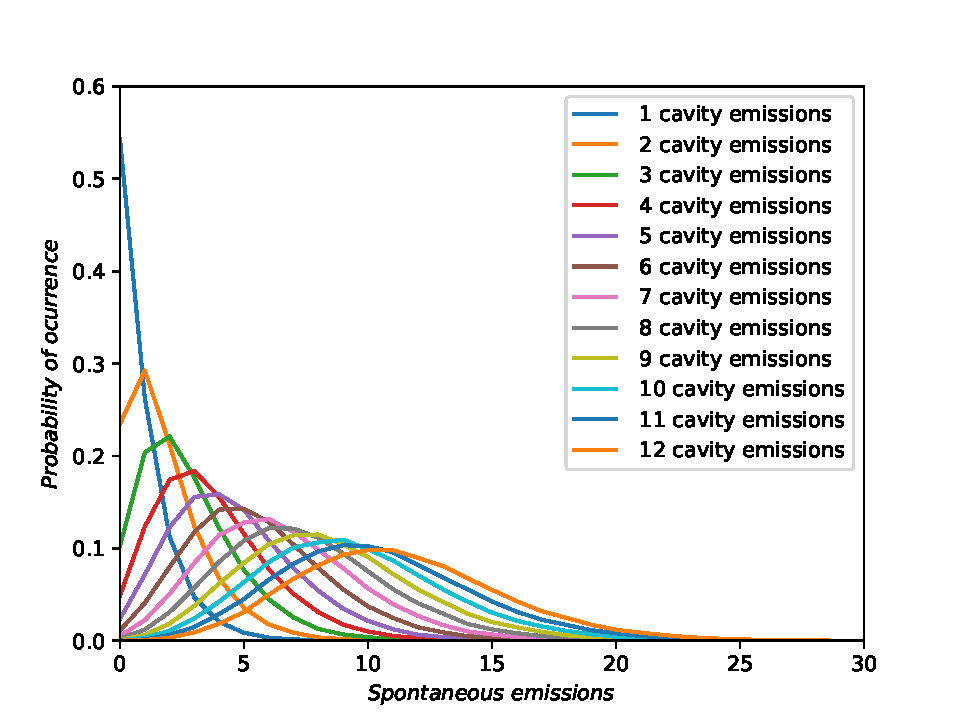
\includegraphics[scale = 0.5]{distributioneng.pdf}
\caption{\small{Probability distribution of spontaneous emissions for different number of cavity losses in a driven Jaynes-cummings model, doing $100,000$ quantum trajectory simulations, with parameters $\mathcal{E}  = \kappa = \gamma = g = 1$.}} \label{probdiss}
\end{figure}
If $\delta p > \epsilon$ is not fulfilled we just renormalize the
state, because using a non-hermitian Hamiltonian will have as a
consequence that the probability won't be conserved
\cite{Sakurai:1167961}. For the next step we repeat the procedure
using the resulting state for this step. One quantum trajectory of
total time $t$ is obtained after repeating the previous procedure
$t/\delta t$ steps. For each trajectory we count the number of quantum
jumps, the jumps correponding to operator $a$ reduces the number of
photons inside the cavity and corresponds to a photon that leak the
cavity. The jumps corresponding to operator $\sigma_-$ interrumps its
unitary evolution and send it back to the ground state, it corresponds
to a spontaneous emission. The procedure to register emissions in the
two different channels is summarized in algorithm. \ref{alg1}.

We realize a large number of these trajectories and keep track of the
numbers of emission for each channel, with this data we can calculate
probability distributions that relate these two quantities.

\section{Counting photons emitted in different channels}\label{sc:distributions}
In this section we calculate the probability distribution of the
number of spontaneous emissions, $n_s$, under different conditions.
First we calculate the distribution probability of $n_s$ when we know
the number of leaked photons from the cavity, $n_c$; we use
$p(n_s|n_c)$ to denote the distribution. Using this function we can
investigate the correlation between $n_s$ and $n_c$ as a function of
the cavity decay rate. This correlation is a measure of how much
information we can obtain about $n_s$ if we know $n_c$.

The number of total photon emissions depends on how fast the atom is
excited. In order to do a meaningful comparison when we change
$\kappa$, we adjust the cavity drive so the mean number of photons
inside the cavity is the same. If we keep $g$ constant this guarantees
that the rate of atomic excitation is the same for different $\kappa$.

In order to find the value of the cavity drive $\mathcal{E}$ as a
function of the mean value of photons inside the cavity, we solve the
Maxwell-Bloch equations. These equations give the dynamic of our
system for the variables $\expval{a}, \expval{\sigma_-}$ and
$\expval{\sigma_z}$ that correspond to the cavity field, atomic
coherence, and atomic inversion respectively \cite{Alsing_1991}. For
the case of the driven Jaynes-Cummings system, these equations are
\begin{subequations} \label{maxbloch}
\begin{equation} \label{bloch1}
\dot{z} = (g/2)v + \mathcal{E} - \kappa z,
\end{equation}
\begin{equation} \label{bloch2}
\dot{v} = gmz - (\gamma/2)v,
\end{equation}
\begin{equation} \label{bloch3}
\dot{m} = -2g(z^*v + v^*z) - \gamma(m + 2),
\end{equation}
\end{subequations} 
where we defined $z = e^{i\omega t}\expval{a}$,
$v = 2e^{i\omega t}\expval{\sigma_-}$ and $m = 2\expval{\sigma_z}$.
When the system is stable, we obtain, from
\eqref{maxbloch}, the steady state
solutions \cite{gagniuc2017markov}
\begin{center}
\begin{figure*}[!t]\label{error2}
\begin{center}
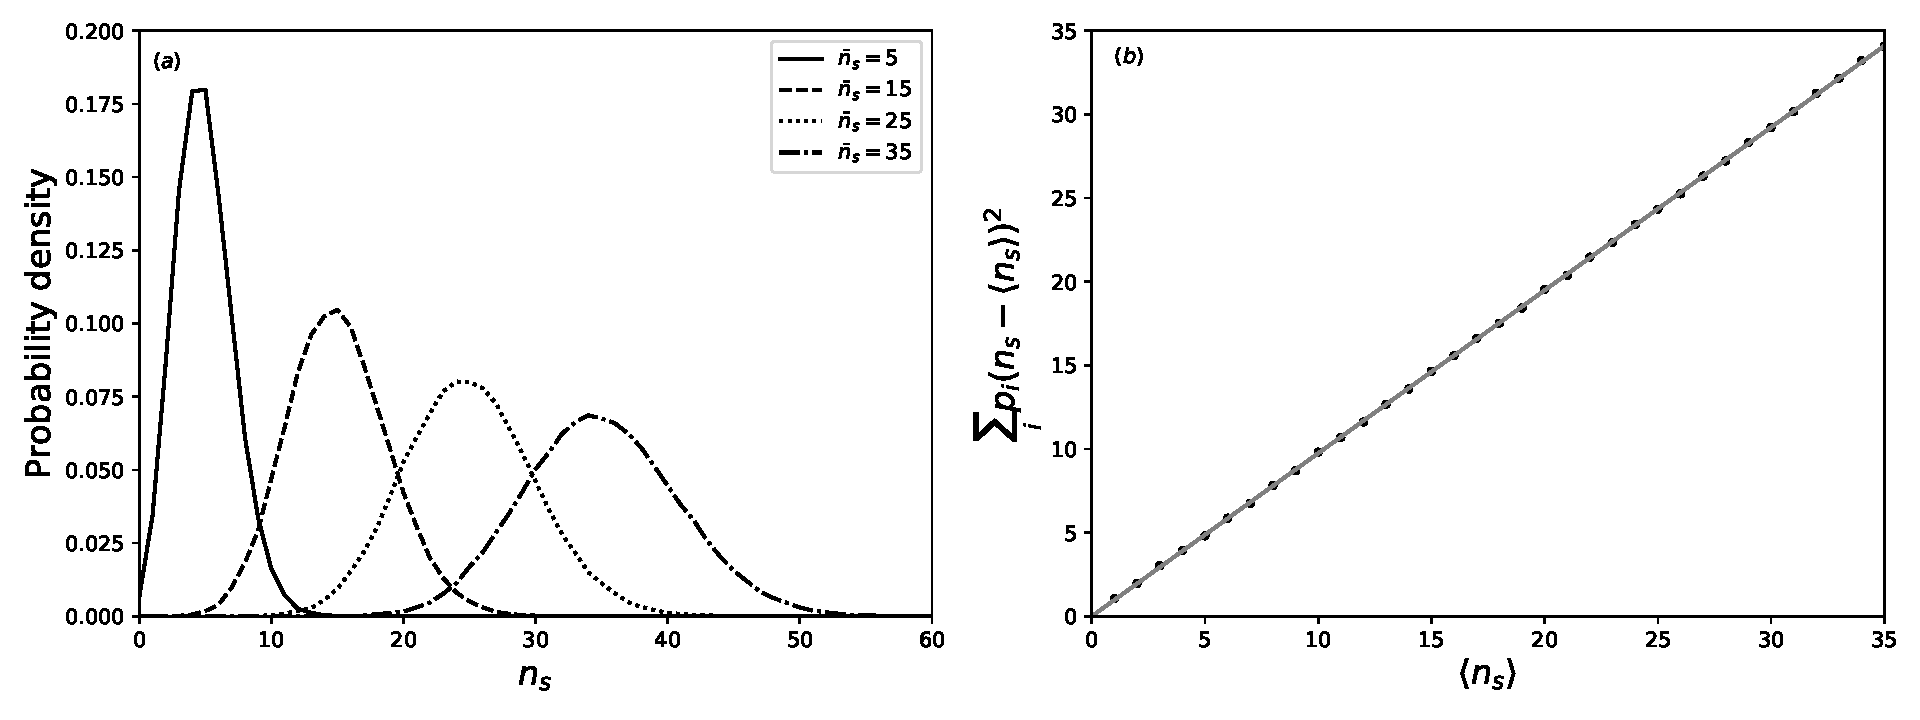
\includegraphics[scale = 0.7]{newerrorppp.pdf}
\caption{\small{(a) Probability distributions for different mean number of spontaneous emissions $\mu$; (b) Calculation of variance with respect to the mean number of sponatenous emissions $\mu$. In both cases we consider $\expval{n} \approx 1$, $\gamma = 1.0$ , $\kappa = g = 0.1$ and $\mathcal{E} =  \kappa |\langle n \rangle|[1 + 2g^2/\gamma \kappa]$.}} \label{probdisult}
\end{center}
\end{figure*}
\end{center}
\begin{equation} \label{chaf1}
\expval{a}_{ss} = \frac{\mathcal{E}e^{-i\omega t} +
  g\expval{\sigma_-}_{ss}}{\kappa}\, ,
\end{equation}
\begin{equation} \label{chaf2}
\expval{\sigma_-}_{ss} = -\frac{2g}{\gamma}\frac{\expval{a}_{ss}}{1 +
  \frac{8g^2}{\gamma^2}|\expval{a}_{ss}|^2}\, ,
\end{equation}
\begin{equation}
\bigg(\frac{\mathcal{E}}{\kappa}\bigg)^2 = |\expval{a}_{ss}|^2 \bigg(1
+ \frac{2g^2}{\gamma \kappa}\frac{1}{1 +
  \frac{8g^2}{\gamma^2}|\expval{a}_{ss}|^2}\bigg)^2\, .
\end{equation}
When $\gamma \gg g$, the expected value of the number of photons in
the cavity is 
\begin{equation} \label{numfo}
|\expval{a}_{ss}|^2 \approx \bigg(\frac{\mathcal{E}/\kappa}{1 + 2g^2/\gamma \kappa}\bigg)^2.
\end{equation}

\paragraph{The case when the number of photons leaked from the cavity  is known}
\fxnote{No esta claro que hiciste aqui. Segun yo corriste el programa
  distinto tiempo para cada caso}
We calculate the distribution probability of the number of spontaneous
emission conditioned to the number of photons detected leaking the
cavity. We assume that the mean flux of photons in each channel is
known in advance (they can be calculated knowing the cavity drive).
The results are shown in Fig.\ref{probdiss}. As the number of leaked
photons increases, the mean number of spontaneous emissions increases.
This result is expected, because the number of leaked photons is
correlated with the time we are counting spontaneus emission photons
from a driven atom: the larger the number of leaked photons the larger
the time we measure spontaneous emitted photons which implies a larger
mean number of emitted photons. Also, the probability distribution is
wider when the number of leaked photons increases, this implies less
accuracy guessing the number of spontaneus emission as the number of
leaked photons increases. If we know the cavity drive, this results
does not imply that we can learn something extra about the number of
spontaneous emissions knowing the number of photons leaked from the
cavity; it is clear that when we increase the time window where we
count photons, both, the number of leaked photons and the number of
spontaneous emissions, increases.

In section~\ref{sc:correlation} we will show
when there is correlation between emissions in the two channels.


\begin{figure}[!b]  
\centering
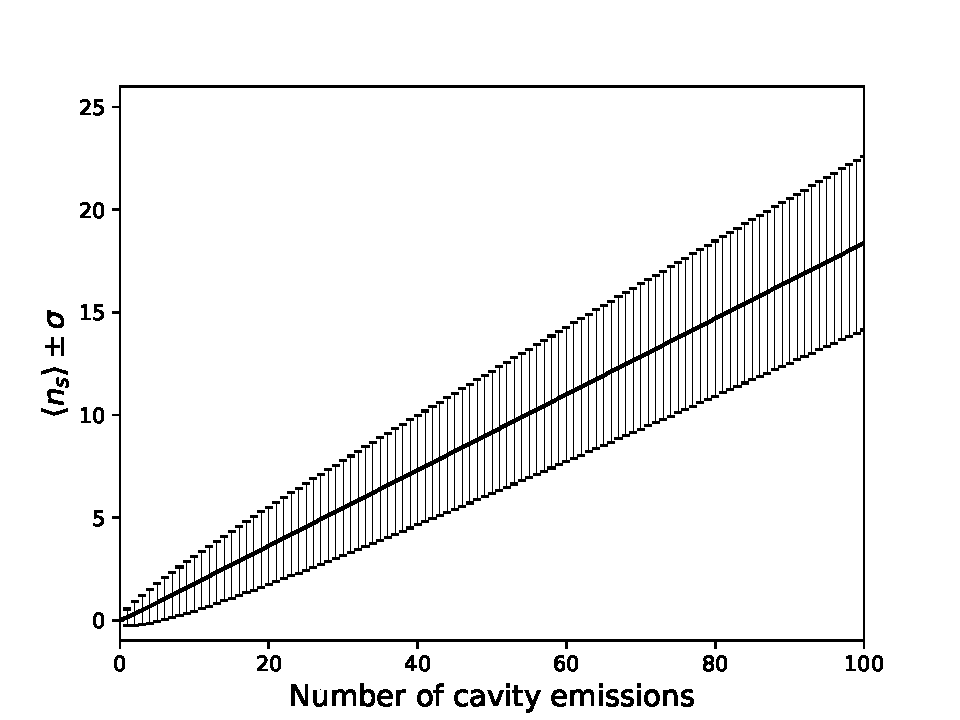
\includegraphics[scale = 0.5]{newsigmaengg.pdf}
\caption{\small{Average number of spontaneous emissions $\pm \sigma$ with respect to cavity emissions, under parameters $\expval{n} \approx 1$, $\gamma = 1$ , $\kappa = g = 0.1$ and $\mathcal{E} =  \kappa |\langle n \rangle|[1 + 2g^2/\gamma \kappa]$.}}
\label{graph}
\end{figure} 


\paragraph{The case where the time we measure photons is fixed}

We know fix the time we measure photons, which is equivalente to
fixing the mean number of spontaneous emited photons or the mean number
of leaked photons from the cavity. 

We focus in the case where we fix the mean number of photons inside
the cavity. This number depends on the cavity drive and the atomic
parameters.


Having Eq. \eqref{numfo} we are able to stablish a dynamic in the system in which we fix the number of photons. Fixing the photon number to one and leaving $\mathcal{E}$ as a free parameter, we obtain probability distributions of the number of spontaneous emissions $E_i$ for different mean number of spontaneous emissions just as we see in Fig. \ref{probdisult} (a). From these probability distributions we can calculate the variance and graph it against the mean value as we see in Fig. \ref{probdisult} (b), where we obtain a variance almost equal to the mean value, something which is characteristic of Poisson distributions. 
Finally we can graph the mean value of spontaneous emissions against the number of cavity emissions considering standard deviation in order to have a better grasp of the certainty in the estimations, something that is shown in Fig. \ref{graph}.


\section{Correlation between photons emitted in different channels}\label{sc:correlation}
In this section we study the correlation between the number of
spontaneus emission from the atom, $n_s$, and the number of photons
that leak the cavity, $n_c$, as a function of the cavity decay rate,
$\kappa$. We expect that when $\kappa\rightarrow\infty$ there would be
no correlation between these two random variables, since this
situation will be equivalent to the situation where there is no
cavity.

In order to have a measure of the correlation between emissions in the
two different channels, we use the Pearson Correlation Coefficient
\cite{benesty2009pearson}
\begin{equation} 
r_{n_s,n_c} = \frac{\sum\limits_{i=1}^n(n_s^{(i)} -
  \bar{n}_s)(n_c^{(i)} - \bar{n}_c)}{\sqrt{\sum\limits_{i=1}^n(n_s^{(i)}
    - \bar{n}_s)^2\sum\limits_{i=1}^n(n_c^{(i)} - \bar{n}_c)^2}}\, ,  \label{correlationc}
\end{equation}
where $n^{(i)}$ is the output $i$ of the random variable $n$.

\begin{center}
\begin{figure}[t!]
\begin{center}
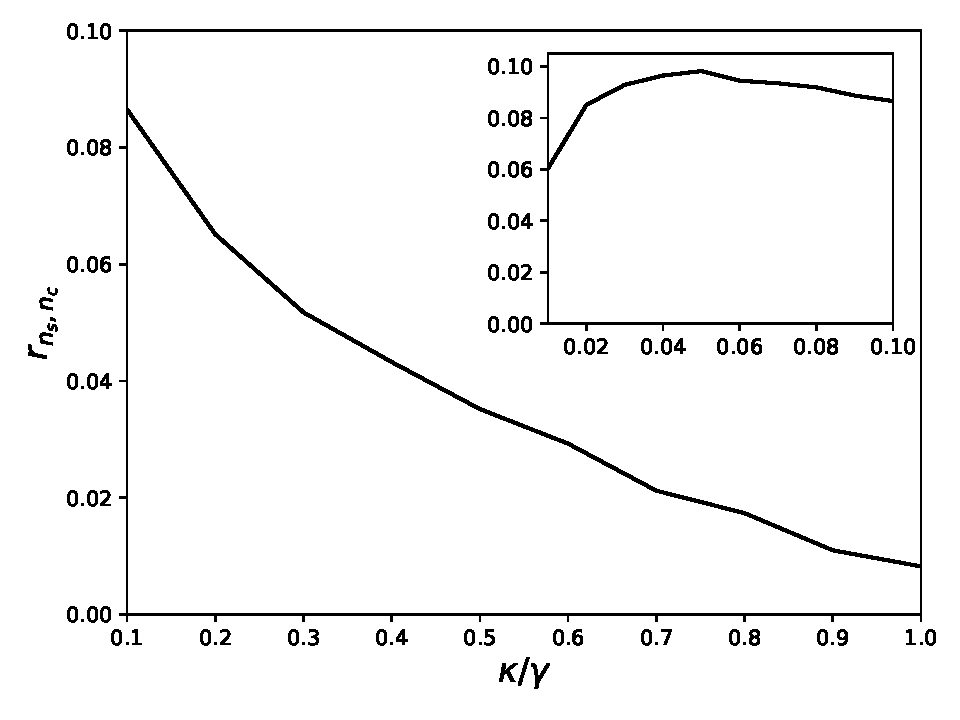
\includegraphics[scale = 0.5]{million1.pdf}
\caption{\small{Calculation of correlation using 500 time intervals, fixing $\expval{n} \approx 1$, $\gamma =$ 1.0, $g = $ 0.1, and with  $\mathcal{E} =  \kappa |\langle n \rangle|[1 + 2g^2/\gamma \kappa]$.}} \label{corrxy}
\end{center}  
\end{figure}
\end{center}

\begin{center}
\begin{figure}[h!]
\begin{center}
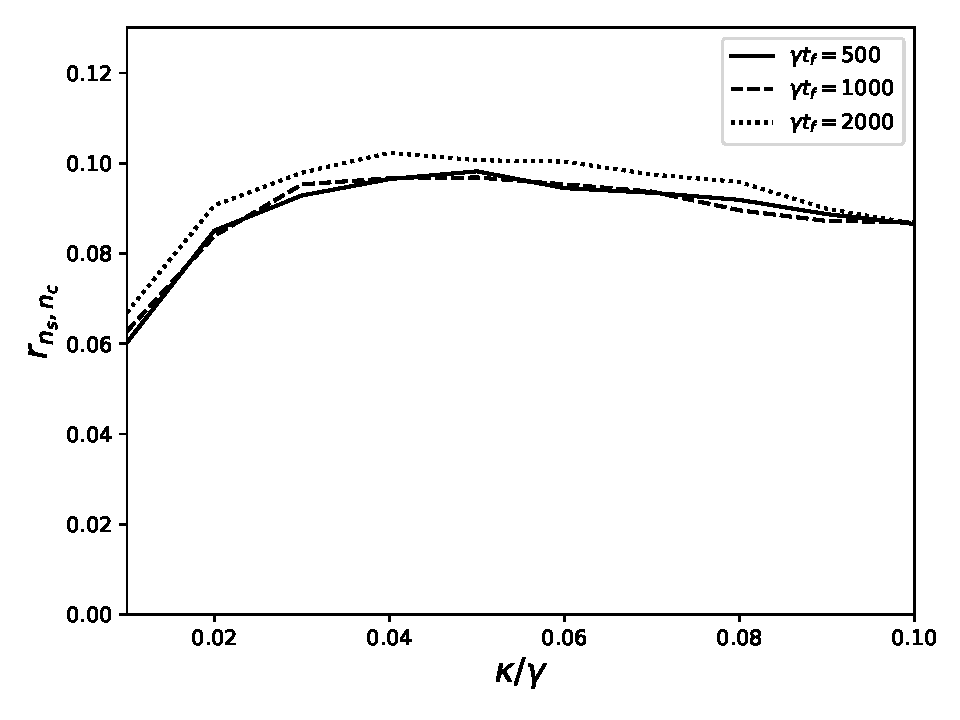
\includegraphics[scale = 0.5]{million2.pdf}
\caption{\small{Correlation using different temporal intervals, fixing $\expval{n} \approx 1$, $\gamma =$ 1.0, $g =$ 0.1, and with  $\mathcal{E} =  \kappa |\langle n \rangle|[1 + 2g^2/\gamma \kappa]$.}}  \label{errorzz}
\end{center}
\end{figure}
\end{center}
%kncrease or increases

\begin{center}
\begin{figure}[h!]
\begin{center}
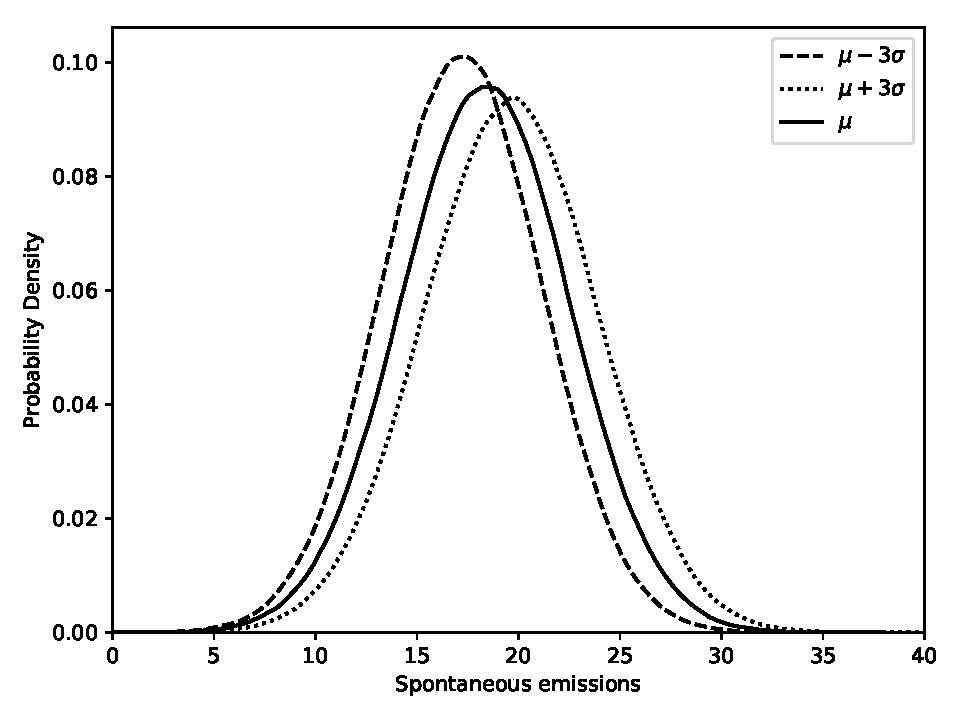
\includegraphics[scale = 0.5]{ccorr1.pdf}
\caption{\small{Mean value of spontaneous emissions after post-selection, fixing $\expval{n} \approx 1$, $\gamma =$ 1.0, $g = \kappa =$ 0.1, and with  $\mathcal{E} =  \kappa |\langle n \rangle|[1 + 2g^2/\gamma \kappa]$.}}  \label{errorzz}
\end{center}
\end{figure}
\end{center}

\begin{center}
\begin{figure}[h!]
\begin{center}
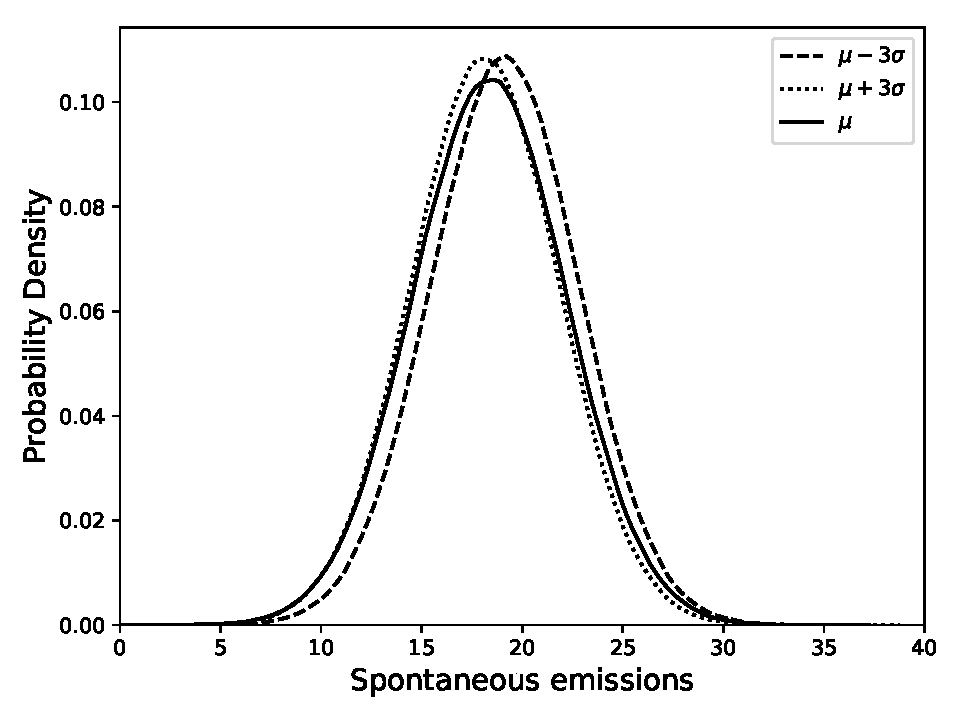
\includegraphics[scale = 0.5]{cnocorr1.pdf}
\caption{\small{Mean value of spontaneous emissions after post-selection, fixing $\expval{n} \approx 1$, $\gamma = \kappa =$ 1.0, $g =$ 0.1, and with  $\mathcal{E} =  \kappa |\langle n \rangle|[1 + 2g^2/\gamma \kappa]$.}}  \label{errorzz}
\end{center}
\end{figure}
\end{center}

The results are shown in Fig. \ref{corrxy}. We see a maximum
correlation close to $0.1$ for $\kappa/\gamma\approx 0.05$ that
decreases as $\kappa$ increases. From the figure it looks like the
correlation goes to zero as $\kappa\rightarrow\infty$. With values for
$\kappa/\gamma$ lower than $0.05$, we notice that the correlations
increase stops and a decrease begins. This stop in the increase of the
correlation is due to the fact that, as we keep decreasing the cavity
linewidth the number of photons that leaks the cavity decreases
considerably. In the limit where $\kappa=0$ the two random
variables becomes independent, because the output of $n_c$ is zero
with probability one. In this case there is no correlation between the two
random variables.





In Fig. \ref{errorzz} it is shown that as we increase the temporal
interval where we count photons, we also see a small increment of the
correlation, due to the fact that more photons leaks the cavity
giving information about the system.
\fxnote{Hay que mejorar las graficas. Las variables tienen que ser
  mayores y las unidades estan mal}

%In Fig. \ref{errorzz} we can appreciate that, as we increase the total temporal interval, the cavity linewidth at which the correlation starts decreasing is smaller. This supports the idea that the time that takes for the system in stablishing the number photons will affect the minimum value of cavity linewidth at which the correlation starts decreasing.



\section{Conclusions}\label{sc:conclusions}
Atomic emission in cavity and non-cavity modes of an atom inside a
leaky cavity are correlated. The correlations are produced because the
cavity breaks the markovian behavior of atomic emission. the presence
of correlation between photons measured in different directions is a
signature of non-markovian behaviour. This correlation also allows us
to improve the knowledge we know about the probability distribution of
atomic spontaneus emission if we know the number of photons that leak
the cavity. 

% In this work we considered a driven Jaynes-Cummings system. We made a
% program in which, through the use of quantum trajectory theory, we
% were able to obtain probability distributions that relate the number
% of spontaneous emissions given certain number of cavity emissions.
% Through the probability distributions we obtained estimations for the
% number of spontaneous emissions by measuring cavity emissions,
% considering the correspondent error. Finally we study the existing
% correlation where we saw how this correlation decreases as we increase
% the cavity linewidth. However, if we try with values for
% $\kappa/\gamma < 0.1$, there comes a point where the increase stops
% and we see a decrease. We believe this is related to the fact that if
% we use enough small values of $\kappa$ there will come a point where
% the emission of photons will be too low and this will imply a decrease
% in the correlation. The results in this work provide a tool that could
% be useful in the manipulation of single photons product of spontaneous
% emission, and provide insight into the physical behavior of the driven
% Jaynes-Cummings model.

\fxnote{Creo que faltan dos cosas en este paper: la correlacion como
  funcion de $g$ dado $\kappa$ constante. Una grafica mostrando, para
  un tiempo fijo, como cambia la funcion de probabilidad para
  emisiones espontaneas como funcion de fotones detectados fuera de la
  cavida. Es decir: $p(n_s,n_c,t_0)$}



\bibliography{reftesis}% Produces the bibliography via BibTeX.

\end{document}
%
% ****** End of file apssamp.tex ******
